% main.tex -- LNCS-format paper skeleton for the Ultrasound Biometry
% Foundation Model work (DINOv2 SSL domain adaptation + HRNet-style neck).
% Based on Springer's llncs.cls / samplepaper.tex (v2.21, 2022/01/12).
%
% Compile with pdflatex + bibtex, e.g.:
%   pdflatex main && bibtex main && pdflatex main && pdflatex main
%
\documentclass[runningheads]{llncs}

\usepackage[T1]{fontenc}
\usepackage{microtype} % better justification/hyphenation -- fixes several
                       % overfull-hbox margin overflows (e.g. long compound
                       % hyphenated words like "task-homogeneous") without
                       % changing any wording
\usepackage{graphicx}
\usepackage{amsmath}
\usepackage{cite} % auto-sorts + range-compresses multi-citations, e.g. [4-6,9]
\usepackage{booktabs}   % clean horizontal-rule tables (\toprule/\midrule/\bottomrule)
\usepackage{multirow}   % multi-row cells (clinical-domain grouping in tab:codabench-results)
\usepackage{subcaption} % side-by-side subfigures, if needed later
\usepackage{xcolor}    % \textcolor{red}{...} -- marks reviewer-driven citation
                        % additions for easy visual revision; remove/plain-ify
                        % once changes are finalized
\raggedbottom           % disable flushbottom's inter-paragraph stretch glue --
                        % without this, sparsely-filled pages (e.g. the
                        % Introduction) visibly space paragraphs further apart
                        % than dense pages, even though the source formatting
                        % is identical
\usepackage{float}      % [H] float placement -- keeps tables/figures exactly
                        % where declared in the source instead of drifting to
                        % the top of a later page (matters while sections are
                        % still placeholder-only with little body text)

% Uncomment for blue, roman-font hyperlinks per Springer's eBook style:
%\usepackage{color}
%\usepackage{hyperref}
%\renewcommand\UrlFont{\color{blue}\rmfamily}
%\urlstyle{rm}

\begin{document}

\title{Self-Supervised Domain Adaptation with DINOv2-HRNet for Multi-Task Ultrasound Landmark Detection}
\titlerunning{SSL Domain Adaptation with DINOv2-HRNet for Ultrasound Landmarks}

\author{Anna Panagiotakopoulou\inst{1}\orcidID{0009-0006-0957-6331}\thanks{Code available at: \texttt{https://github.com/abarmper/US-Foundation}} \and
Alexandros Barmperis\inst{1,2}\orcidID{0009-0000-6319-0700} \and
Vasileios E. Katsigiannis\inst{1}\orcidID{0009-0003-7464-0959} \and
George K. Matsopoulos\inst{1}\orcidID{0000-0002-2600-9914}}

\authorrunning{A. Panagiotakopoulou et al.}

%\institute{Your Institution, City, Country\\
\institute{Biomedical Engineering Laboratory, School of Electrical and Computer Engineering, \\
National Technical University of Athens, Athens, Greece\\
%\email{you@institution.edu}}
\email{annapan@biomed.ntua.gr, amparmperis@biomed.ntua.gr,
vassiliskat@biomed.ntua.gr, gmatsopoulos@biomed.ntua.gr} \and
Archimedes Research Unit, Athena Research Center, Athens, Greece}

\maketitle

\begin{abstract}
Accurate ultrasound biometry relies on precise anatomical landmark localization, yet building a unified model across heterogeneous ultrasound tasks remains challenging. Image appearance, acquisition protocols, and anatomical scale vary substantially across clinical domains, exacerbated by the severe scarcity of large-scale annotated datasets. To address the Generalization-oriented Ultrasound Biometry Challenge, we propose a two-stage foundation-model pipeline for generalizable multi-task landmark detection across nine diverse clinical tasks. Rather than treating each task as an isolated problem, we formulate biometry as cross-domain representation learning under limited keypoint supervision and distribution shift. First, a DINOv2 encoder is adapted to unlabeled ultrasound through multi-crop self-distillation combining CLS-level DINO supervision, masked patch-token prediction, and KoLeo regularization under an EMA teacher, capturing domain-specific sonographic textures. Second, the adapted encoder is coupled with a domain-agnostic, HRNet-style multi-resolution neck designed to reconstruct localization-relevant spatial hierarchies directly from transformer patch features. Task-specific convolutional heads then utilize soft-argmax for direct, sub-pixel coordinate regression. {\color{blue}On the official evaluation, our pipeline achieves an overall MRE of 35.03\,px and MAE of 34.62\,px across all nine tasks.}

\keywords{Ultrasound biometry \and Self-supervised learning \and DINOv2 \and
Landmark localization \and HRNet.}
\end{abstract}


\section{Introduction}
Ultrasound biometry converts a small set of anatomical landmarks into clinically meaningful measurements, such as fetal biometric parameters~\cite{salomon2019isuog}, labor progression indices~\cite{ghi2018isuog,ramirez2025intrapartum}, and cardiac structural measurements~\cite{mitchell2019comprehensive}. Landmark localization has been studied extensively with single-task models~\cite{avisdris2022biometrynet,bai2026iugc,zhou2020aop,lu2022aop,bai2025landmarkchallenge}, but multi-centre benchmarks reveal that site and scanner variability substantially degrades generalization~\cite{bai2026beyond,divece2026multicentre}. This heterogeneity renders task-specific supervision insufficient, motivating the need for a unified pipeline that can preserve spatial accuracy and measurement reliability under the cross-domain distribution shift central to the challenge (GU\_Biometry)~\cite{gu_biometry,deng2026baseline}.

Foundation models have advanced medical image analysis through reusable representation learning from unlabeled data: self-supervised transformers like DINOv2 learn transferable visual features without manual labels~\cite{oquab2023dinov2}, though direct transfer to sonography remains challenging given ultrasound's distinct texture statistics, acquisition physics, and artifacts~\cite{guan2022domain}. Recent ultrasound foundation models~\cite{jiao2024usfm,ambsdorf2025general,lin2025uusic} motivate domain-specific pretraining, but primarily target image-level classification, dense prediction, or few-shot analysis, leaving unified sparse landmark localization across biometric domains underexplored.

Landmark-based biometry requires global context alongside fine spatial precision. Vision Transformers extract robust features~\cite{dosovitskiy2021image,oquab2023dinov2} and have been adapted for keypoints (e.g., TransPose~\cite{yang2021transpose}, ViTPose~\cite{xu2022vitpose}). However, their coarse tokenization reduces native spatial resolution, making precise coordinate localization more challenging; even hierarchical variants such as Swin~\cite{liu2021swin} rely on progressive downsampling. We therefore pair foundation model features with a High-Resolution Network (HRNet)-style multi-resolution neck~\cite{sun2019hrnet}, preferred over standard U-Net architectures to maintain continuous high-resolution spatial detail throughout the network, critical for fine coordinate estimation.

Our main contributions are: (i) a two-stage DINOv2-HRNet pipeline that separates domain-level ultrasound representation learning from task-specific spatial localization; (ii) a study of how unlabeled self-supervised learning (SSL) adaptation duration affects downstream landmark accuracy; (iii) an internal macro-averaged, per-task-normalized validation strategy for checkpoint selection across heterogeneous tasks.

\section{Methodology}

\begin{figure}[tb]
\centering
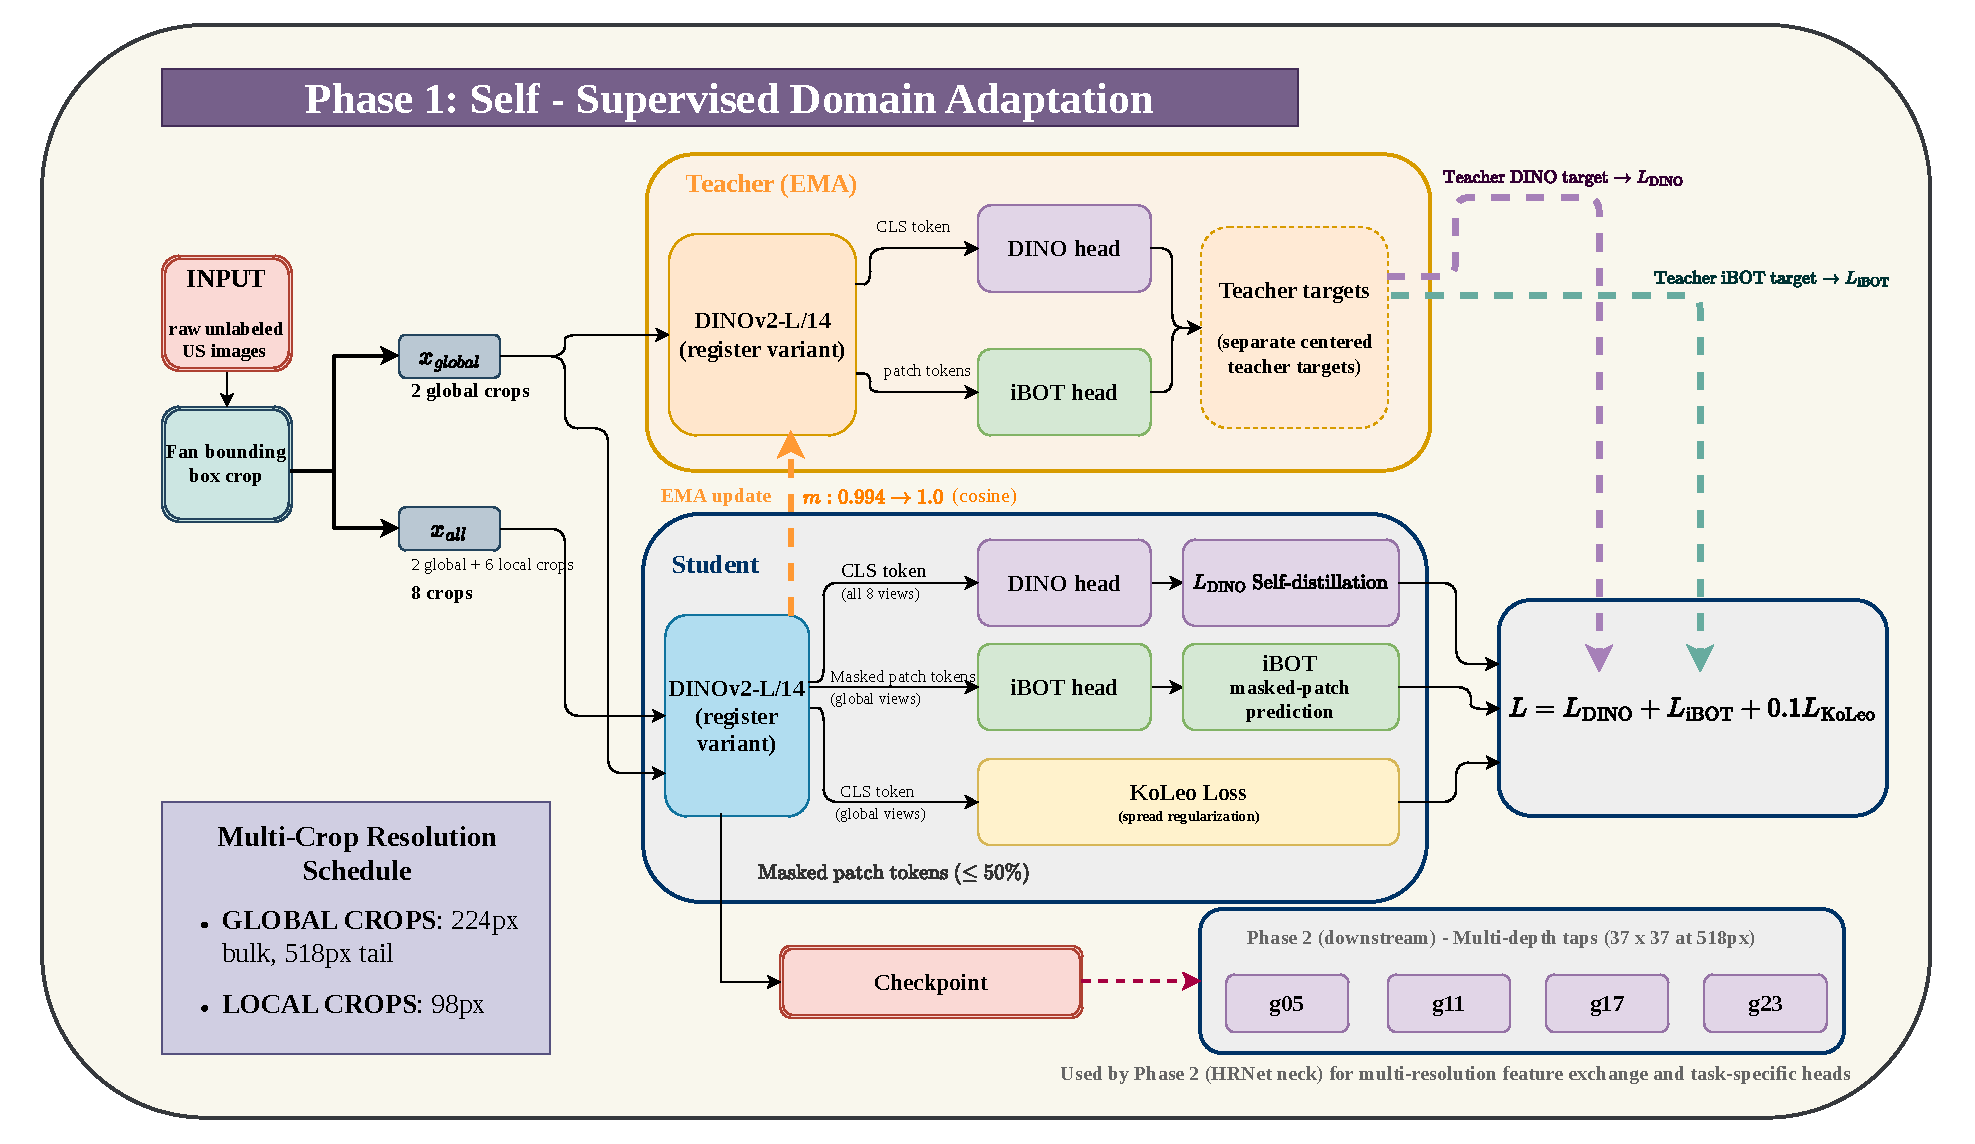
\includegraphics[width=\textwidth]{figures/fig1_phase1_pipeline.pdf}
\caption{{\color{blue}Phase 1 self-supervised domain adaptation.}}
\label{fig:pipeline}
\end{figure}

\subsection{Phase 1: Self-Supervised Domain Adaptation}
\label{sec:phase1}

{\color{blue}
We adapt the register-variant DINOv2-L/14 encoder~\cite{oquab2023dinov2} to unlabeled ultrasound frames with a continued-pretraining recipe that follows DINOv2's original SSL formulation, combining CLS-token self-distillation~\cite{caron2021dino}, masked patch-token prediction~\cite{zhou2022ibot}, and an entropic spread regularizer~\cite{sablayrolles2018spreading}. A local-to-global multi-crop strategy generates eight augmented views: two \emph{global} crops ($224\times224$) and six \emph{local} crops ($98\times98$). A trainable student processes all eight views; an exponential-moving-average (EMA) teacher processes only the two global views.

The DINO branch projects the CLS token through a projection head~\cite{oquab2023dinov2} into $K$ prototypes; the iBOT branch applies an architecturally identical head, separately parameterized, to patch-token representations from the global views. The teacher's logits are centered and sharpened before distillation, following standard DINO self-distillation~\cite{caron2021dino}, now applied independently to both the CLS-level and patch-level heads. In addition to the CLS-level loss $\mathcal{L}_{\mathrm{dino}}$, a block-wise, foreground-restricted subset of the student's global-crop patch tokens is masked and passed through a second head; the student must recover the teacher's representation for each masked patch, giving a dense, patch-level loss:
\begin{equation}
\mathcal{L}_{\mathrm{ibot}} = -\frac{1}{|\mathcal{M}|}\sum_{m\in\mathcal{M}} q_m \log p_m ,
\label{eq:ibot-loss}
\end{equation}
where $\mathcal{M}$ is the set of masked foreground patches across the two global crops, $q_m$ the teacher's centered target and $p_m$ the student's prediction for patch $m$. A Kozachenko--Leonenko entropic term $\mathcal{L}_{\mathrm{koleo}}$~\cite{sablayrolles2018spreading} additionally penalizes overly similar CLS embeddings within a batch, discouraging representational collapse independently of the centering mechanism. The three terms combine as
\begin{equation}
\mathcal{L} = \mathcal{L}_{\mathrm{dino}} + \mathcal{L}_{\mathrm{ibot}} + 0.1\,\mathcal{L}_{\mathrm{koleo}} .
\label{eq:dino-combined}
\end{equation}

The teacher receives no gradient and is updated via an exponential moving average of the student. Pretraining follows a two-resolution curriculum: the bulk of training runs at a low $224\times224$ global-crop resolution, followed by a short high-resolution adaptation tail at $518\times518$---the resolution used by Phase 2---so the encoder's features are finally tuned at the deployment scale rather than only at the cheap pretraining scale. We use $K{=}65{,}536$ prototypes, anneal the teacher temperature from $0.04$ to $0.07$ over the first 30 epochs, freeze the final projection layer during the first epoch, and maintain an effective batch size of 256 through gradient accumulation.
}

\subsection{Phase 2: Multi-Stage HRNet Neck}
\label{sec:phase2}
To recover fine spatial resolution from the coarse $37\times37$ transformer tokens, we implement a multi-stage HRNet-style neck: parallel, multi-resolution branches that repeatedly exchange information bidirectionally (Figure~\ref{fig:neck-zoom}).

\begin{figure}[tb]
\centering
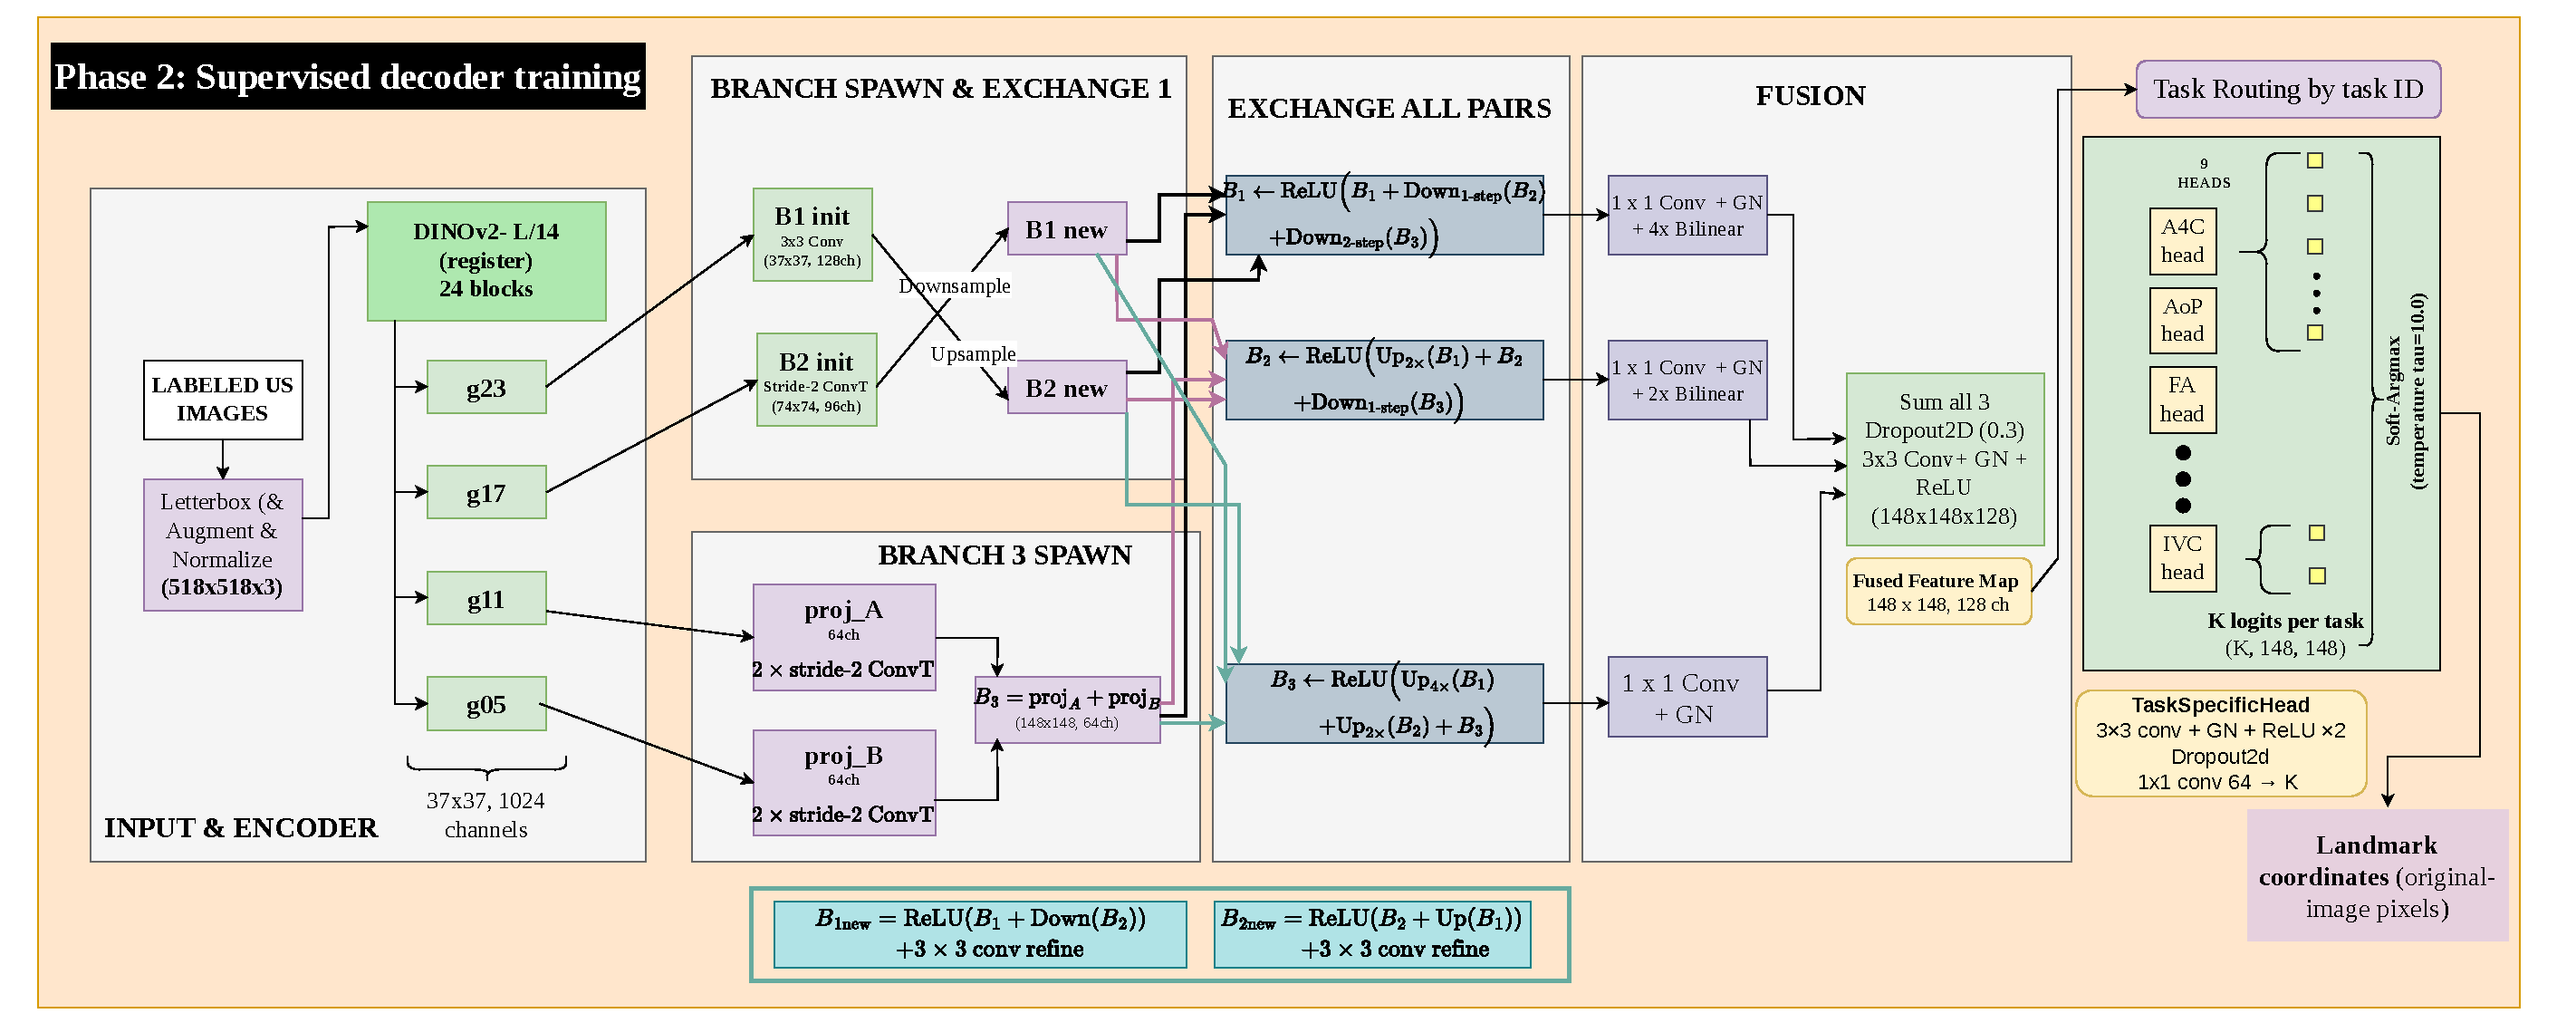
\includegraphics[width=\textwidth]{figures/fig2_hrnet_neck.pdf}
%\caption{Detailed view of Phase 2 (expanding the "Neck" and "Regression" black boxes of Fig.~\ref{fig:pipeline}): branch spawning, the two exchange units, and the final multi-scale fusion into a $148\times148$, 128-channel representation, followed by task routing, the nine task-specific heads, and soft-argmax coordinate decoding.}
\caption{Phase~2 architecture: HRNet-style branch spawning and exchange, fusion into a $148\times148$, 128-channel map, task-routed heads, and soft-argmax decoding.}
\label{fig:neck-zoom}
\end{figure}

Given a $518\times518$ input, the adapted register-variant DINOv2-L/14 encoder outputs, at every one of its 24 transformer blocks, a $37\times37$ grid of 1024-dimensional patch tokens. We tap four intermediate depths---blocks 5, 11, 17, and 23---and route them into three branches at $37\times37$/128ch, $74\times74$/96ch, and $148\times148$/64ch, respectively. Two exchange stages follow---first between the two coarser branches, then a dense all-pairs exchange across all three---using stride-2 convolution downsampling, $1\times1$-projection-plus-bilinear-interpolation upsampling, and GroupNorm throughout (chosen over BatchNorm since training batches are task-homogeneous, so BatchNorm statistics would blend across nine heterogeneous task distributions). The three branches are finally fused into a common $148\times148$, 128-channel representation.

\subsection{Task-Specific Heads and Coordinate Extraction}
Each task-homogeneous batch is routed by its sampler-provided task identity to one of nine independent task-specific heads. Each head applies two Conv-GroupNorm-ReLU blocks with 2D dropout and predicts per-keypoint logits $\ell_k$ through a final $1\times1$ projection.

Coordinates are then extracted via soft-argmax, a temperature-scaled softmax over the flattened logits treated as a differentiable spatial expectation~\cite{nibali2018numerical}:
\begin{equation}
p_k = \text{softmax}(\tau \cdot \ell_k), \qquad
(\hat{x}_k, \hat{y}_k) = \Big(\sum_{(u,v)} p_k(u,v)\, u,\ \sum_{(u,v)} p_k(u,v)\, v\Big) \cdot \frac{518}{H},
\label{eq:softargmax}
\end{equation}
with temperature $\tau=10.0$ and $H$ the logit resolution ($148$). At inference, predictions are inverse-letterboxed to original-image pixels, matching the coordinate space used for validation and official evaluation. Training uses a masked $L_1$ loss over annotated keypoints, reweighted by each image's letterbox scale factor so residuals are measured in original-pixel units matching the metric's scale, together with a light DSNT-style regularizer~\cite{nibali2018numerical}.

%%%%%%%%%%%%%%%%%%%%%%%%%%%%%%%%%%%%%%

\section{Experiments}
\subsection{Dataset and Preprocessing}
We evaluate on the GU\_Biometry dataset~\cite{gu_biometry,bai2026fugc}, spanning multi-vendor 2D ultrasound across three clinical domains (intrapartum, prenatal, and cardiac) and nine distinct biometric tasks, each defining landmarks for a different clinical measurement. The released training data comprise 197{,}938 images in total: 6{,}768 labeled and 191{,}170 unlabeled (a $\sim$3.4\% labeled fraction). Both pools are highly imbalanced across tasks: labeled counts range from 4{,}000 (AoP) to under 100 (IVC, PLAX, PSAX), and unlabeled counts are similarly skewed---fetal femur has none at all. For supervised training, the labeled set is split 80\%/20\%, yielding 5{,}414 training and 1{,}354 validation images.

Native image sizes vary substantially across tasks (e.g., median $336\times544$ for FUGC to $768\times1024$ for FA); to preserve landmark geometry for the DINOv2 encoder, all images undergo an aspect-ratio-preserving resize and zero-padding to a $518\times518$ canvas, followed by ImageNet pixel normalization. On top of this base preprocessing, both phases use common intensity augmentations such as brightness/contrast, gamma/CLAHE, and blur/noise. Phase~2 additionally uses affine transformations, while {\color{blue}Phase~1 uses ultrasound-specific foreground cropping, milder rotations, and resampling of background-heavy local crops.} Validation and inference use only the base preprocessing, with no augmentation.

\subsection{Implementation Details}
All experiments were executed on a single NVIDIA A100-SXM4-80GB GPU with a batch size of 64. Training uses bf16 mixed precision with gradient-norm clipping and AdamW (weight decay excluded on norm/bias parameters, dimensionality $<2$; base LR $2\times10^{-4}$, 15-epoch linear warmup, 150-epoch cosine decay). The backbone uses layer-wise learning rate decay (LLRD, factor $0.75$), starting at $0.1\times$ base LR for the last four unfrozen blocks. A Phase~2 EMA teacher ($\alpha=0.999$) is maintained for stabilized validation, early stopping (patience 40), and final inference. A temperature-scaled ($\tau=0.5$) task-homogeneous sampler allocates per-task batches in proportion to the square root of task size, so that AoP, despite having 82 times more labeled images than PSAX, is seen only 9 times as often per epoch. Checkpoint selection uses an internal macro-averaged, per-task-normalized development criterion combining landmark and clinical-measurement error in original-pixel space, which we refer to below as the \emph{blend} score (lower is better). We use this criterion solely for internal model selection on the held-out validation split; final performance is reported separately using the official Codabench MRE/MAE in Table~1. {\color{blue}Phase~1 (351.7M parameters, fully trained) runs at 64.4~img/s (224px bulk) and 15.9~img/s (518px tail), $\sim$96 GPU-hours in total; Phase~2 (312.2M parameters, 58.2M trainable) trains at 84.4~img/s and infers at up to 127.3~img/s under bf16 autocast.}

%%%%%%%%%%%%%%%%%%%%%%%%%%%%%%%%%%%%%%%%%%%

\section{Results}

% ============================================================
% Results narrative: two cheap fold-0 searches, then one final
% validated 5-fold+TTA run. Steps 1-2 use the LOCAL scorer
% (metrics.py, verified to reproduce official local_eval) on
% fold 0's held-out split -- no Codabench submissions spent on
% search. Step 3 is the official Codabench submission.
% ============================================================

\subsection{Official Challenge Evaluation}
{\color{blue}We report the official evaluation first, with the Phase-1 and Phase-2 choices behind it justified by the ablations in Sections~\ref{sec:ssl-duration} and~\ref{sec:phase2-recipe} that follow.} Using the best Phase-1 checkpoint (Table~\ref{tab:phase1-phase2}) and the upgraded Phase-2 recipe, we submit a single model to the official Codabench evaluation (Table~\ref{tab:codabench-results}), where performance varies substantially across domains due to anatomy, data scarcity, and annotation structure. Figure~\ref{fig:best-per-task} illustrates localization on four representative tasks.

\begin{table}[tb]
\caption{Official GU\_Biometry Codabench evaluation per task.}
\label{tab:codabench-results}
\centering
\begin{tabular}{llrrr}
\toprule
\textbf{Clinical domain} & \textbf{Task / Target view} & \textbf{$N$} & \textbf{MRE $\downarrow$} & \textbf{MAE $\downarrow$} \\
\midrule
\multicolumn{5}{l}{\textbf{Prenatal \& Gynecologic}} \\
 & Head Circumference (HC) & 215 & 45.20 & 59.64 \\
 & Fetal Abdomen (FA)      & 188 & 28.38 & 89.30 \\
 & Fetal Femur             & 62  & 27.38 & 18.24 \\
 & Cervical Segm. (FUGC)   & 20  & 13.79 & 10.63 \\
\midrule
\multicolumn{5}{l}{\textbf{Intrapartum}} \\
 & Angle of Progression (AoP) & 60 & 16.97 & 8.26 \\
\midrule
\multicolumn{5}{l}{\textbf{Cardiac \& Vascular}} \\
 & Parasternal Long (PLAX)  & 26 & 24.83 & 14.85 \\
 & Apical 4-Chamber (A4C)   & 20 & 40.62 & 27.99 \\
 & Parasternal Short (PSAX) & 18 & 82.29 & 60.87 \\
 & Inferior Vena Cava (IVC) & 10 & 35.82 & 21.84 \\
\midrule
\textbf{Overall Summary} & \textbf{Unweighted Average} & \textbf{619} & \textbf{35.03} & \textbf{34.62} \\
\bottomrule
\end{tabular}
\end{table}

% TODO: fig_best_per_task_row.pdf below is still from the OLD/legacy model.
% Regenerate it from the final single-model (winning Phase-1 checkpoint +
% upgraded Phase-2 recipe) model's actual predictions before submission.
\begin{figure}[tb]
\centering
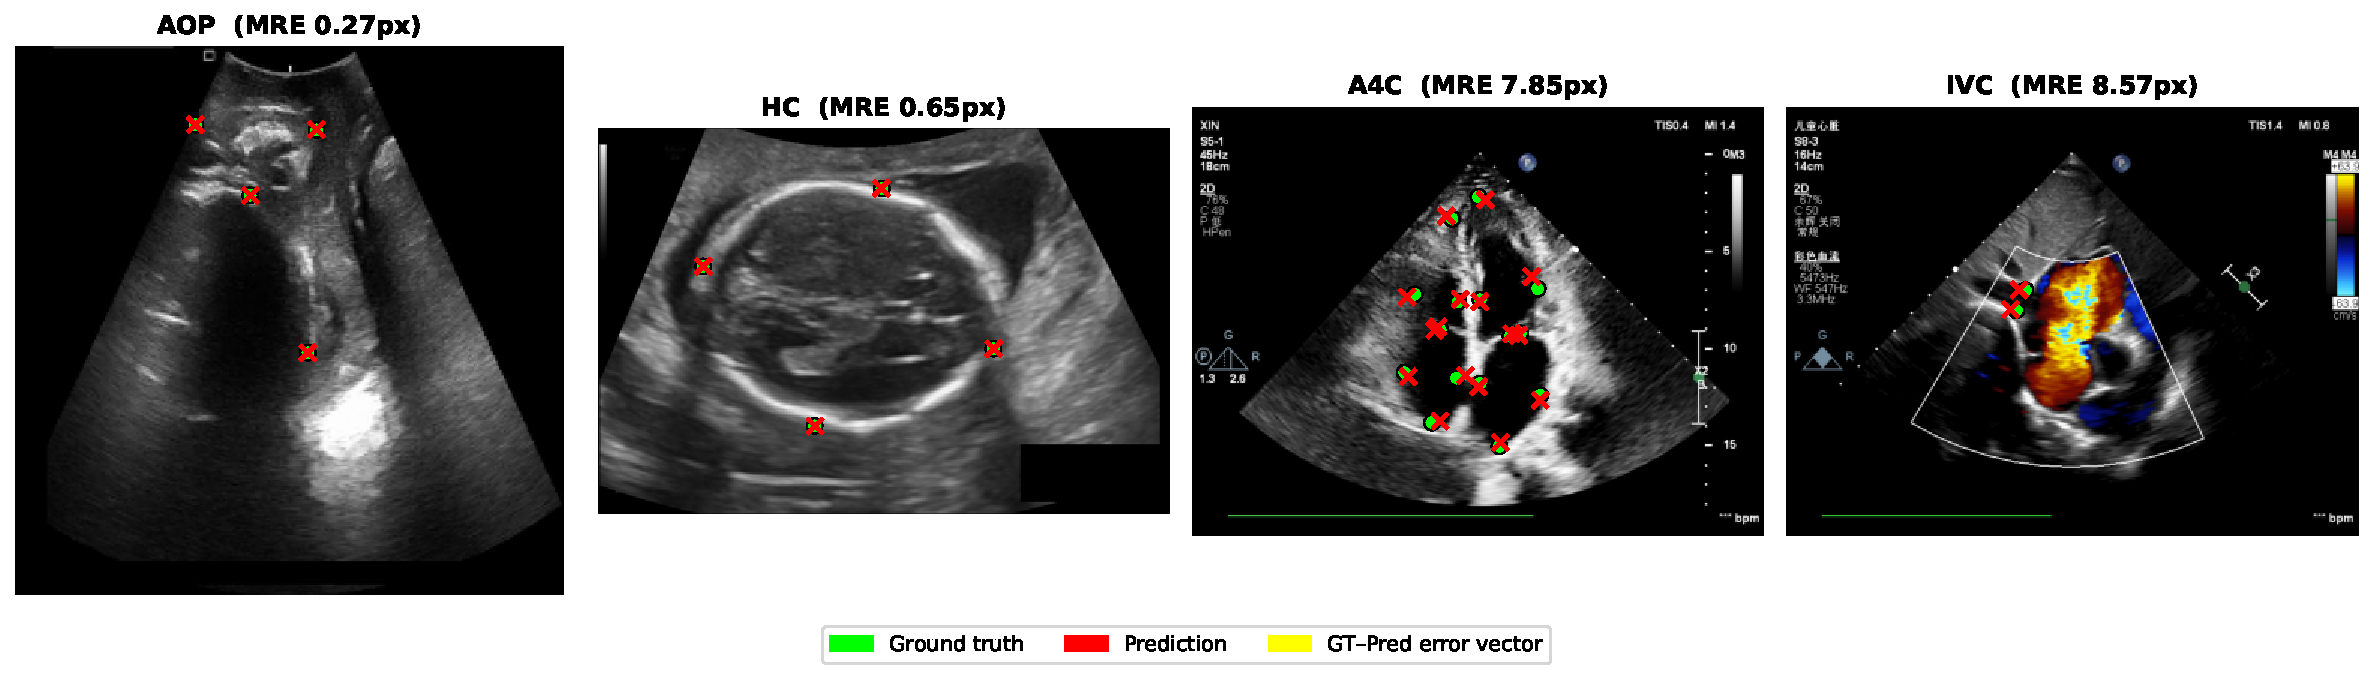
\includegraphics[width=\textwidth]{figures/fig3_best_per_task.pdf}
\caption{Representative high-performing validation examples for four tasks spanning different clinical domains. Ground-truth (green) vs.\ predicted (red) keypoints.}
\label{fig:best-per-task}
\end{figure}

\subsection{Phase-1 Checkpoint Duration Selection}
\label{sec:ssl-duration}

{\color{blue}
To isolate representation quality from downstream fine-tuning, we evaluate
each Phase-1 checkpoint with a frozen-encoder probe. The DINOv2 encoder is
fixed (\texttt{unfreeze}=0), while an identical downstream localization
model is trained for 25 epochs on fold~0 using the same multi-level neck,
$148\times148$ output resolution, and task-homogeneous sampler. Thus, only
the encoder initialization varies across runs. Probe results are used
solely to compare relative representation quality on the internal fold-0
validation split and are not directly comparable with the fully fine-tuned
models reported elsewhere in the Results section.

Figure~\ref{fig:ssl-duration} sweeps SSL duration under this protocol
against an off-the-shelf, non-adapted DINOv2 control (blend 0.0890, MRE
31.27~px). Downstream probe performance is non-monotonic with adaptation
duration (panel a): the ep20 bulk-only MRE optimum (24.70~px) is not
improved by further bulk-only training, and by ep100 the blend score is
worse than the non-adapted baseline (0.0974 vs.\ 0.0890) --- this
non-monotonic behavior suggests that prolonged adaptation does not
necessarily translate into improved downstream localization. A short
518px tail improves the later bulk checkpoints and yields the best probe
blend score of any checkpoint tested (100~ep~+~4-ep tail, blend 0.0747),
though its MRE (25.09) does not surpass the ep20 bulk-only MRE optimum. At
a matched 20-epoch duration, full-resolution adaptation (panel b) does not
improve on 224-pixel bulk training (25.96 vs.\ 24.70~px), supporting the
low-resolution-bulk-then-tail curriculum. The lowest aggregate probe MRE is
obtained at ep20, whereas ep104 achieves the best blend score and completes
the 224-to-518-pixel resolution curriculum. We therefore select ep104 as
the final Phase-1 initialization. Task-specific optima range from ep20 to
ep104, although ep104 remains within 8\% MRE of the per-task optimum for
eight of nine tasks.
}

\begin{figure}[tb]
\centering
\subcaptionbox{224px bulk-only + high-res tail\label{fig:ssl-duration-a}}{%
  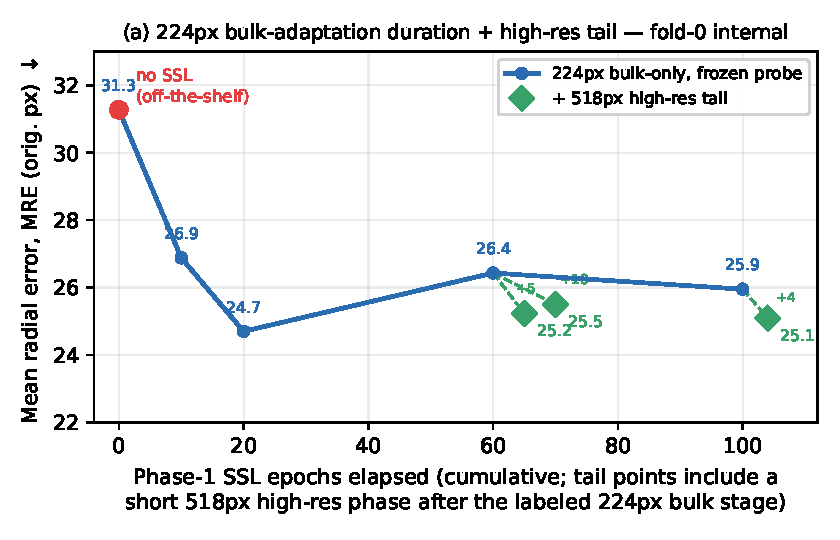
\includegraphics[width=0.48\textwidth]{figures/fig4a_ssl_duration_224.pdf}}
\hfill
\subcaptionbox{518px full-resolution control\label{fig:ssl-duration-b}}{%
  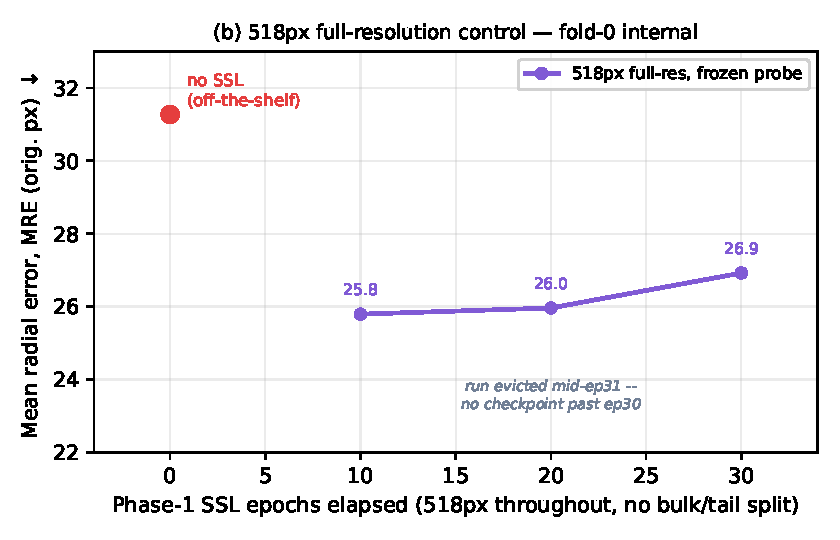
\includegraphics[width=0.48\textwidth]{figures/fig4b_ssl_duration_fullres.pdf}}
\caption{\color{blue}Frozen-encoder probe: MRE (orig.\ px) vs.\ Phase-1 SSL
adaptation duration, fold-0 internal validation. (a) 224px bulk-only
checkpoints (0/10/20/60/100 epochs) plus tail-appended variants. (b) 518px
full-resolution-throughout control.}
\label{fig:ssl-duration}
\end{figure}

\begin{figure}[H]
\centering
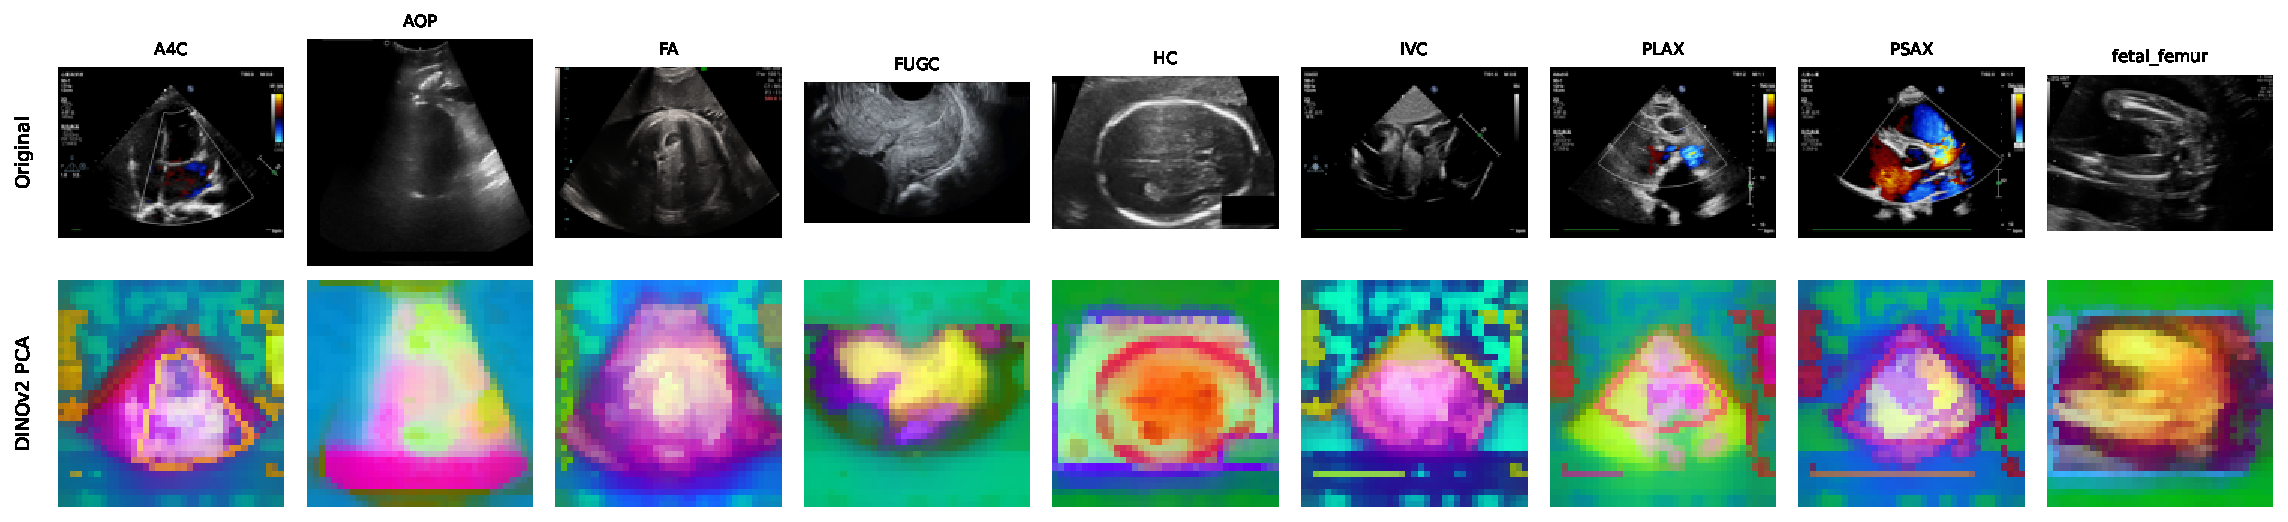
\includegraphics[width=\textwidth]{figures/fig5_pca_ep104.pdf}
\caption{{\color{blue}DINOv2 patch-token PCA features at the selected ep104 checkpoint, across all nine tasks.}}
\label{fig:feature-maps}
\end{figure}

{\color{blue}
\textbf{Register-token ablation.} A matched probe comparison produced mixed
results: registers improved the blend score (0.0890 vs.\ 0.0976), whereas
the standard backbone achieved lower MRE (29.34 vs.\ 31.27~px). We therefore
retain registers primarily for their reported ability to suppress high-norm
artifact tokens in intermediate ViT features~\cite{darcet2024registers},
which is relevant because our neck directly consumes dense patch
representations.
}

\subsection{Phase-2 Recipe Selection}
\label{sec:phase2-recipe}
The Phase-1 initialization is fixed at the epoch-10 checkpoint. To isolate the Phase-2-specific upgrades from the backbone choice, both configurations use the register-variant backbone. We then compare the baseline Phase-2 recipe (single-mode neck, $128\times128$ heatmap, without LLRD, canvas-space loss, without DSNT) against the upgraded recipe (multilevel neck, $148\times148$ heatmap, LLRD $0.75$, original-pixel loss, DSNT $0.1$), on fold~0 only with the same local scorer. Table~\ref{tab:phase1-phase2} reports the results, where the upgraded recipe improves both MRE and AvgMAE and is carried forward to the final model.

\begin{table}[tb]
\caption{Fold-0 internal validation: Phase-1 checkpoint duration (left, baseline recipe) and Phase-2 recipe (right, epoch-10 checkpoint), side by side. Mean radial error (MRE, px) and mean absolute clinical-measurement error (AvgMAE), macro-averaged over all nine tasks.}
\label{tab:phase1-phase2}
\centering
\begin{tabular}{@{}lcc|lcc@{}}
\toprule
Phase-1 checkpoint & epoch 10 & epoch 20 & Phase-2 recipe & Baseline & Upgraded \\
\midrule
Mean MRE & 40.32 & \textbf{33.95} & Mean MRE & 40.32 & \textbf{31.12} \\
Mean AvgMAE & 25.33 & \textbf{23.37} & Mean AvgMAE & 25.33 & \textbf{22.52} \\
\bottomrule
\end{tabular}
\end{table}

\section{Conclusion}
We presented a two-stage DINOv2-HRNet pipeline for multi-task ultrasound landmark detection, coupling domain-targeted self-supervised adaptation with a top-down, multi-resolution HRNet-style neck to achieve competitive performance across nine heterogeneous clinical tasks. Future work includes a stratified 5-fold ensemble with multi-scale/intensity test-time augmentation, and ablating the neck's multi-level fusion, head design, and fine-tuning depth.

\begin{credits}
\subsubsection{\ackname} % Funding / acknowledgments, if any.
The A100 80GB GPU cloud instances (MedViLA) used to train and evaluate all models in this study were provided by the NVIDIA Academic Hardware Grant Program.
\subsubsection{\discintname}
The authors have no competing interests to declare that are relevant to
the content of this article.
\end{credits}

%
% ---- Bibliography ----
% BibTeX users: specify bibliography style 'splncs04' (Springer's LNCS
% style). Entries live in mybibliography.bib next to this file.
%
\bibliographystyle{splncs04}
\bibliography{mybibliography}

\end{document}
